\documentclass[a4paper, 12pt]{article}%тип документа

%отступы
\usepackage[left=2cm,right=2cm,top=2cm,bottom=3cm,bindingoffset=0cm]{geometry}

%Русский язык
\usepackage[T2A]{fontenc} %кодировка
\usepackage[utf8]{inputenc} %кодировка исходного кода
\usepackage[english,russian]{babel} %локализация и переносы

%Вставка картинок
\usepackage{wrapfig}
\usepackage{graphicx}
\graphicspath{{pictures/}}
\DeclareGraphicsExtensions{.pdf,.png,.jpg}

%оглавление
\usepackage{titlesec}
\titlespacing{\chapter}{0pt}{-30pt}{12pt}
\titlespacing{\section}{\parindent}{5mm}{5mm}
\titlespacing{\subsection}{\parindent}{5mm}{5mm}
\usepackage{setspace}

%Графики
\usepackage{multirow}
\usepackage{pgfplots}
\pgfplotsset{compat=1.9}

%Математика
\usepackage{amsmath, amsfonts, amssymb, amsthm, mathtools}

%Стиль страницы
\usepackage{fancyhdr}
\pagestyle{fancy}

\begin{document}

\begin{titlepage}

\begin{center}
%\vspace*{1cm}
\large\textbf{Московский Физико-Технический Институт}\\
\large\textbf{(государственный университет)}
\vfill
\line(1,0){430}\\[1mm]
\huge\textbf{Работа 4.3.1.}\\
\line(1,0){430}\\[1mm]
\vfill
\large Сибгатуллин Булат, ФРКТ\\
\end{center}

\end{titlepage}
\fancyhead[L] {Работа 4.3.1.}
\noindent \textbf{Цель работы:} \\
\indent Исследовать дифракцию Френеля на узкой щели, на краю экрана, на тонкой нити; исследовать дифракцию Фраунгофера на щели и проследить, как влияют изменение ширины щели и её смещение на характер дифракционной картины; исследовать картину дифракции на двух щелях и оценить влияние размеров источника на чёткость картины; исследовать влияние дифракции на разрешающую способность оптических инструментов.\\
\noindent \textbf{В работе используются:} \\
\indent оптическая скамья, ртутная лампа, монохроматор, щели с регулируемой шириной, рамка с вертикальной нитью, двойная щель, микроскоп на поперечных салазках с микрометрическим винтом, зрительная труба.

\section*{Теоретическое введение и установка}
	\subsection*{А. Дифракция Френеля}
	
	Схема установки для наблюдения дифракции Френеля представлена на рис. 1. Световые лучи освещают щель~$S_2$ и испытывают на ней дифракцию. Дифракционная картина рассматривается с помощью микроскопа~М, сфокусированного на некоторую плоскость наблюдения~П.
		\begin{figure}[h]
		\begin{center}
			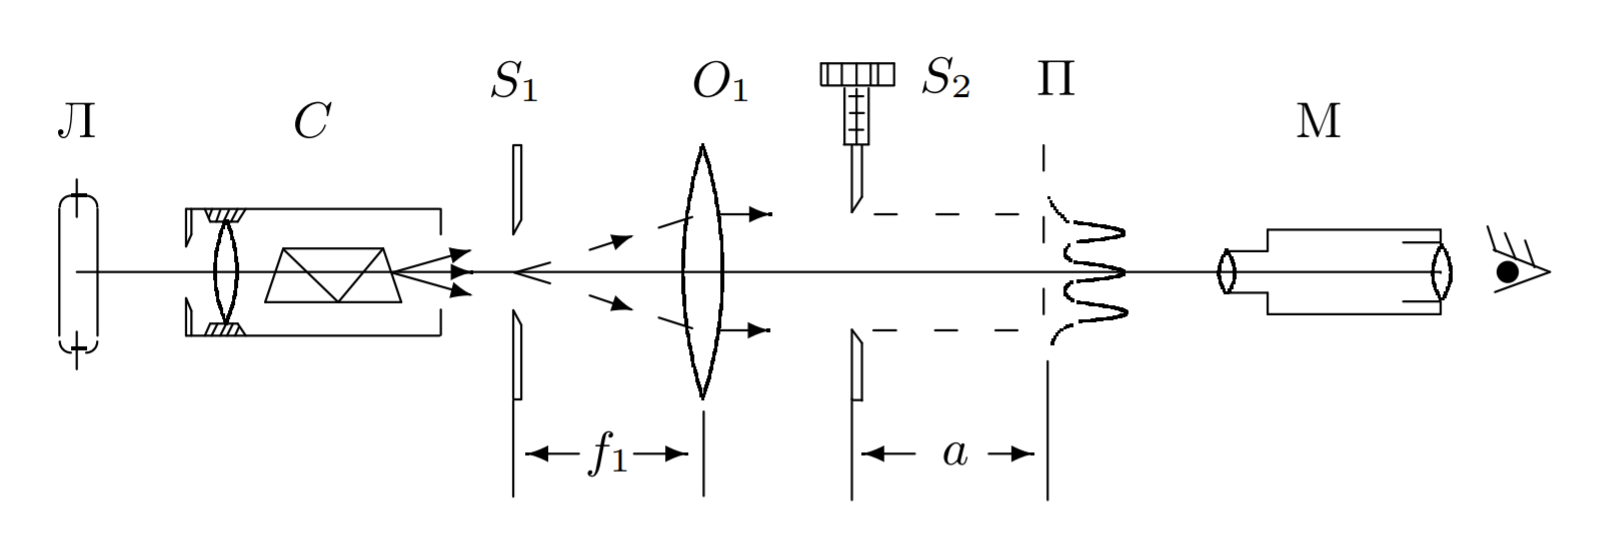
\includegraphics[width = 0.7\textwidth]{images/431-1.png}
			\caption{Схема установки для наблюдения дифракции Френеля}
		\end{center}
	\end{figure}
	
	Щель~$S_2$ освещается параллельным пучком монохроматического света с помощью коллиматора, образованного объективом~$O_1$ и щелью~$S_1$, находящейся в его фокусе. На щель~$S_1$ сфокусировано изображение спектральной линии, выделенной из спектра ртутной лампы~Л при помощи простого монохроматора~C.
	
	
	Распределение интенсивности света в плоскости наблюдения~П проще всего рассчитывать с помощью зон Френеля (для щели их иногда называют зонами Шустера). При освещении щели~$S_2$ параллельным пучком лучей (плоская волна) зоны Френеля представляют собой полоски, параллельные краям щели (рис. 2). Результирующая амплитуда в точке наблюдения определяется суперпозицией колебаний от тех зон Френеля, которые не перекрыты створками щели. Графическое определение результирующей амплитуды производится с помощью векторной диаграммы --- спирали Корню. Суммарная ширина $m$ зон Френеля $z_m$ определяется соотношением
	\begin{equation}
	z_m=\sqrt{am\lambda},
	\end{equation}
	где $a$ --- расстояние от щели до плоскости наблюдения (рис. 1), а $\lambda$ --- длина волны.
	
	Вид наблюдаемой дифракционной картины определяется числом Френеля $\Phi$: квадрат числа Френеля
	\begin{equation*}
	\Phi^2 = \dfrac{D}{\sqrt{a\lambda}}.
	\end{equation*}
	Дифракционная картина отсутствует, когда плоскость наблюдения~П совпадает с плоскостью щели: при $\Phi \rightarrow \infty$ мы имеем дело с геометрической оптикой. При небольшом удалении от щели, когда число Френеля $\Phi \gg 1$ (на щели укладывается огромное число зон), дифракционная картина наблюдается только в узкой области на границе света и тени у краёв экрана.
	
	При последующем небольшом удалении от щели (или изменении ширины щели $S_2$) эти две группы дифракционных полос перемещаются практически независимо друг от друга. При дальнейшем увеличении расстояния (или уменьшении ширины щели~$S_2$) обе системы дифракционных полос постепенно сближаются и, наконец, при $\Phi \gtrsim 1$ накладываются друг на друга. Распределение интенсивности в плоскости наблюдения в этом случае определяется числом зон Френеля, укладывающихся на полуширине щели. Если это число равно $m$, то в поле зрения наблюдается $n=m-1$ тёмных полос. Таким образом, по виду дифракционной картины можно оценить число зон Френеля на полуширине щели.

	\subsection*{Б. Дифракция Фраунгофера на щели}
	\begin{wrapfigure}{r}{0.5\textwidth}
		\begin{center}
			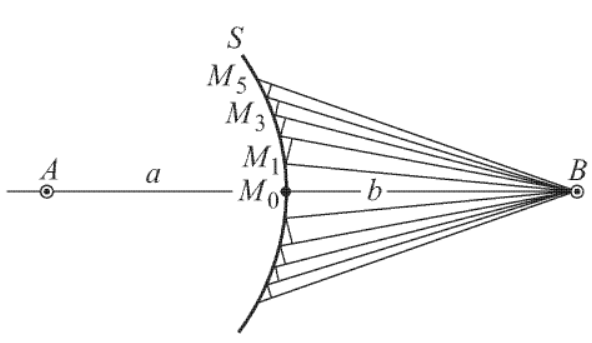
\includegraphics[width = 0.4\textwidth]{images/431-2.png}
		\end{center}
		\caption{Построение зон Френеля}
	\end{wrapfigure}
	Принцип Гюйгенса-Френеля:\\
	\textit{Каждый элемент волнового фронта можно рассматривать как центр  вторичного возмущения, порождающего вторичные сферические волны, а результирующее световое поле  в каждой точке пространства будет определяться интерференцией этих волн.}\\
	Теперь рассмотрим первое применение этого принципа, получившее название \textit{метод зон Френеля}
	

	Для этого рассмотрим действие световой волны действующей из точки $A$ в какой-то точке $B$.
	В этом случае можно, взяв точку $M_0$ в качестве центра (см. рис. 1), построить ряд концентрических сфер, радиусы которых начинаются с $b$ и увеличиваются каждый раз на половину длины волны $\frac{\lambda}{2}$. При пересечении с плоским фронтом волны $F$ эти сферы дадут концентрические окружности. Таким образом, на фронте волны появятся кольцевые зоны (зоны Френеля) с радиусами $r_1, r_2$ и т. д.
	
	Из геометрических соображений посчитав, можно получить, что 
	\begin{equation}
	r_i = i \sqrt{a \lambda}.
	\end{equation}
		\begin{wrapfigure}{r}{0.3\textwidth}
		\begin{center}
			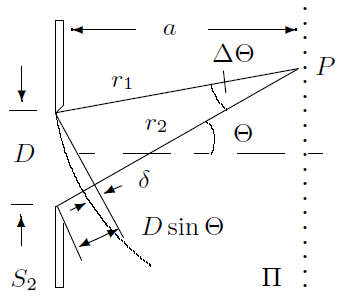
\includegraphics[width = 0.3\textwidth]{images/431-3.png}
		\end{center}
		\caption{К фазовым соотношениям при дифракции Фраунгофера}
	\end{wrapfigure}
	
	Картина дифракции упрощается, когда ширина щели становится значительно меньше ширины первой зоны Френеля, т.е. если 
	\begin{equation}
	D \ll\sqrt{a \lambda} 
	\end{equation}	
	Это условие всегда выполняется при достаточно большом $a$. В этом случае говорят, что \textit{дифракция Фраунгофера}. Дифракционную картину в этом случае называются \textit{дифракцией Фраунгофера}. При выполнении пункта $(2)$ у нас упрощаются фазовые соотношения, что поясняет рис. 2, в итоге с хорошим приближением можно считать, что разность хода между крайними лучами, приходящими от щели в точке наблюдения $P$, с хорошим приближением равна 
	\begin{equation}
	\Delta = r_2 - r_1 \approx D \sin \theta \approx D \cdot \theta
	\end{equation}
	Здесь предполагается, что $\theta$ достаточно мал.
	Дифракцию Фраунгофера можно наблюдать на установке рис. 1, но для удобства к подобной установке добавляется объектив $O_2$.
	
	\begin{figure}[h]
		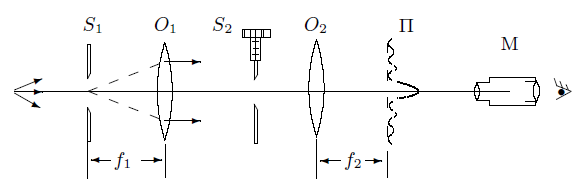
\includegraphics[width = 0.7\textwidth]{images/431-4.png}
		\centering
		\caption{Схема установки 2.}
	\end{figure}
	Дифракционная картина здесь наблюдается в фокальной плоскости объектива $O_2$. Каждому значению $\theta$ соответствует в этой плоскости точка, отстоящая от оптической оси на расстоянии 
	\begin{equation}
	X = f_2 \tan \theta \approx f_2 \theta.
	\end{equation}
	Объектив не вносит разности хода между интерферирующими лучам, поэтому в его фокальной плоскости наблюдается неискажённая дифракционная картина. При $\theta = 0$ разность хода между лучами нулевая, поэтому в центре поля зрения дифракционный максимум. Первый минимум соответствует $\theta_1$ такому, что в точке наблюдения разность хода пробегаем все значения от 0 до $2\pi$. Аналогично рассуждая, для $m$-й полосы
	\begin{equation}
	\theta_m = \frac{m \lambda}{D}
	\end{equation}
	Расстояние $X_m$ тёмной полосы от оптической оси из (5) и (6)
	\begin{equation}
	X_m = f_2m\frac{\lambda}{D}
	\end{equation}
	\subsection*{В. Дифракция Фраунгофера для двух щелей}
	Для наблюдения дифракции Фраунгофера на двух щелях $S_2$ заменим экраном Э с двумя щелями. При этом для оценки влияния ширины входной щели на чёткость вместо $S_1$ поставим щель с микрометрическим винтом.
	\begin{figure}[h]
		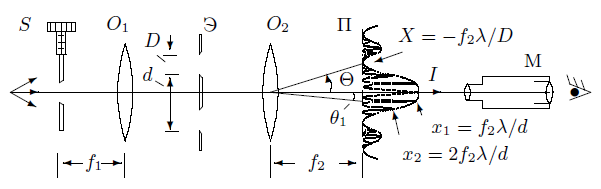
\includegraphics[width = 0.7\textwidth]{images/431-5.png}
		\centering
		\caption{Схема установки В.}
	\end{figure}
	Два дифракционных изображения входной щели, одно из которых образовано лучами, прошедшими через левую, а другое -- через правую щели, накладываются друг на друга.
	Если входная щель достаточно узка, то дифракционная картина в плоскости П подобна той, что получалась при дифракции на одной щели, однако вся картинка испещерена рядом дополнительных узких полос, наличие которых объясняется суперпозицией световых волн через разные щели. Светлая интерфереционная полоса наблюдается в случаях, когда разность хода равна целому числу длин волн. Таким образом, угловая координата максимума порядка $m$ равна
	\begin{equation}
	\theta_m = \dfrac{m \lambda}{d},
	\end{equation}
	где $d$ -- расстояние между щелями. Отсюда расстояние между соседними интерфереционными полосами в плоскости П равно
	\begin{equation}
	\delta x = f_2 \dfrac{\lambda}{d}
	\end{equation}
	Число интерференционных полос укладывающихся в области центрального максимума равна отношению ширины главного максимума $\frac{2\lambda f_2}{D}$ к расстоянию между соседними полосами:
	\begin{equation}
	n = \dfrac{2\lambda f_2}{D} \dfrac{1}{\delta f}= \dfrac{2d}{D}.
	\end{equation}
	При дифракции света на двух щелях чёткая система интерференционных полос наблюдается только при достаточно узкой ширине входной щели $S$. При увеличении ширины картинка пропадает и появляется вновь, но полосы при этом сильно размыты и видны плохо.
	\subsection*{Г. Влияние дифракции на разрешающую способность оптического инструмента}
	\begin{figure}[h]
		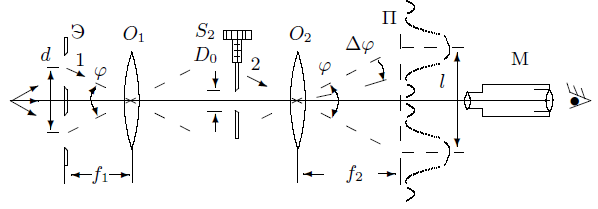
\includegraphics[width = 0.8\textwidth]{images/431-6.png}
		\centering
		\caption{Схема установки 4.}
	\end{figure}
	В отсутствие щели $S_2$ линзы $O_1$ и $O_2$ создают на плоскости П изоюражение щели $S_1$ и это изображение рассматриваются микроскопом М. Таким образом, установку можно рассматривать как оптический инструмент, предназначенные для получения изображения предмета. Если перед $O_2$ расположить $S_2$, то изображение объекта будет искажено из-за дифракции. Чем меньше ширина щели, тем сильнее искажение. Качественной характеристикой этого искажения может служить $\varphi_{min}$ --- минимальное угловое расстояние между объектами (источниками), которые всё ещё воспринимаются как раздельные. Поместим вместо $S_1$ экран Э с двумя щелями с расстоянием $d$. Тогда на $S_2$ будут падать два пучка света с углом
	\begin{equation}
	\varphi = \dfrac{d}{f_1}
	\end{equation}
	Из геометрии расстояние $l$ между изображениями щелей в плоскости П равно 
	\begin{equation}
	l = \varphi f_2 = d \dfrac{f_2}{f_1}.
	\end{equation}
	Ширина $\Delta \varphi$ определяется дифракцией на $S_2$. Условия, при которых изображения различимы разные для разных наблюдателей, поэтому используют \textit{критерий Рэлея} -- \textit{максимум одного дифракционного пятна должен совпадать с минимумом другого}. В наших условиях это значит, что угловая полуширина $\frac{\lambda}{D}$ равна угловому расстоянию $\frac{l}{f_2}$.
	
\section*{Ход работы}

\subsection*{А}

\begin{enumerate}

\item Соберем схему изображенную на рис. 1 и настроим ее. Получим изображение темных и светлых полос в микроскопе.

\item Передвигая микроскоп по шкале продольной линейки получим четкое изображение щели:

\[x = 49,60 \pm 0,05 \: \text{см}\]

Постепенно отодвигая микроскоп от щели $S_2$, заметим по шкале положение микроскопа, при котором на фоне щели видна одна темная полоса. Приближая микроскоп к щели снимем зависимость координаты микроскопа от числа n наблюдаемых темных полос:

\begin{center}
\begin{tabular}{|c|c|}
\hline 
n & x, см \\ 
\hline 
1 & 47,6 \\ 
\hline 
2 & 48,2 \\ 
\hline 
3 & 48,6 \\ 
\hline 
4 & 48,8 \\ 
\hline 
5 & 49 \\ 
\hline 
6 & 49,1 \\ 
\hline 
\end{tabular} 
\end{center} 

\item Построим график зависимости размера зоны Френеля от количества теных полос:

\begin{figure}[h]
		\begin{center}
			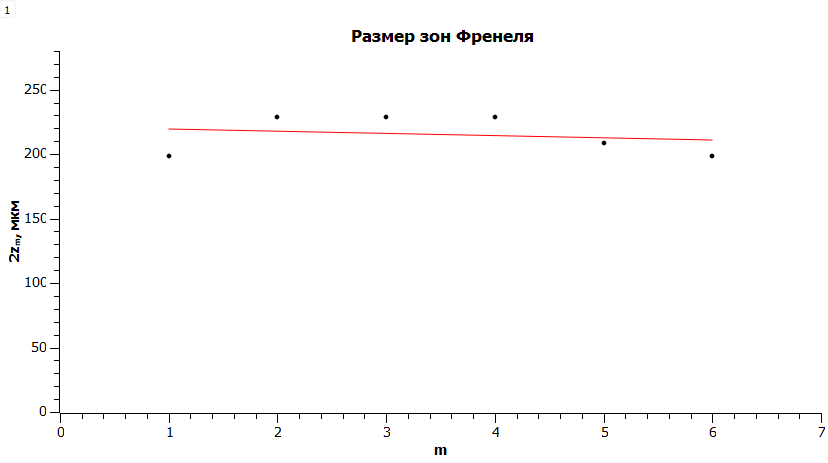
\includegraphics[width = 0.7\textwidth]{images/graph_!.png}
			\caption{Размер зон Френеля}
		\end{center}
	\end{figure}
	
Получаем, что усредненное значение размера зоны Френеля равен:

\[2z_m = 221 \pm 17 \: \text{мкм}\]

\item Измерим ширину D щели $S_2$ :

\[D = 226 \pm 0,5 \: \text{мкм}\]

Получаем, что размер щели примерно совпадает с шириной щели.

\item Закрепим миксроскоп на оптической скамье и проследим за изменением дифракционной картины при уменьшении ширины щели $S_2$. В результате получим, что чем меньше щель, тем меньше количество полос.

\end{enumerate}

\subsection*{Б}

\begin{enumerate}

\item Соберем схему изображенную на рис. 4 и настроим ее. Получим изображение темных и светлых полос в микроскопе.

\item С помощью винта поперечного измерения микроскопа координаты $X_m$ нескольких дифракционных минимумов:

\begin{center}
\begin{tabular}{|c|c|}
\hline 
m & $X_m,$ мкм \\ 
\hline 
-2 & 200 \\ 
\hline 
-1 & 520 \\ 
\hline 
0 & 880 \\ 
\hline 
1 & 1160 \\ 
\hline 
2 & 1520 \\ 
\hline 
\end{tabular} 
\end{center}

Построим график по получившимся данным и получим зависимость вида $y = ax + b$, где:

\[a= 328 \pm 7 \quad b = 856 \pm 9\]

\begin{figure}[h]
		\begin{center}
			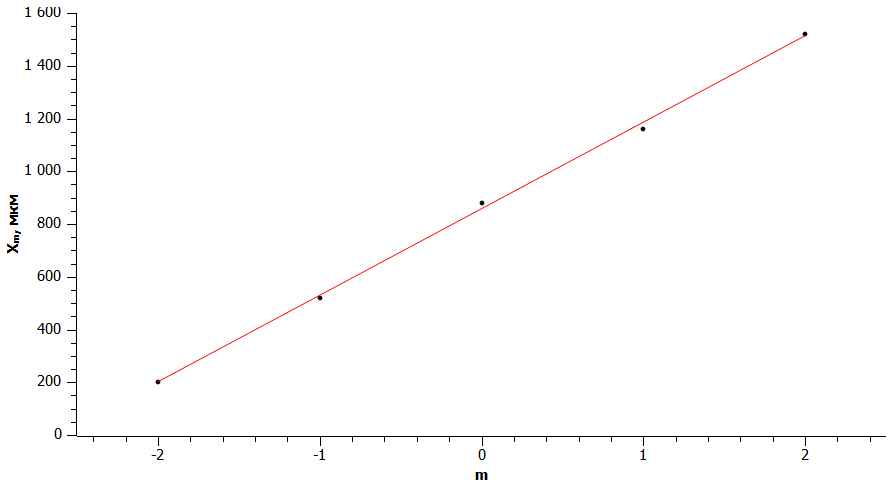
\includegraphics[width = 0.7\textwidth]{images/graph_2.png}
			\caption{Координаты минимумов дифракции Фраунгофера}
		\end{center}
	\end{figure}

\item Учтем погрешности измерения и запишем, чему равно $\bigtriangleup X$:

\[\bigtriangleup X = 328 \pm 23 \: \text{мкм}\]

\item Пользуясь полученным результатом и зная, что $f_2 = 12,5$ см, получим значение D c помощью формулы (7):

\[D = 208 \pm 15 \: \text{мкм}\]

\item Измерим ширину щели по показаниям микрометрического винта:

\[D = 212 \: \text{мкм}\]

Видим, что измеренные величины совпадают в пределах погрешности.

\end{enumerate}

\subsection*{В}

\begin{enumerate}

\item Соберем схему изображенную на рис. 5 и настроим ее. Получим изображение темных и светлых полос в микроскопе.

\item Измерим ширину щели:

\[D = 212 \pm 1 \: \text{мкм}\]

\item Получим на экране дифракционную картину и проведем измерения для дифракционных максимумов аналогично предыдущему пункту:

\begin{center}
\begin{tabular}{|c|c|}
\hline 
m & $X_m$, мкм \\ 
\hline 
-2 & 28 \\ 
\hline 
-1 & 32 \\ 
\hline 
-1 & 101 \\ 
\hline 
-2 & 106\\ 
\hline 
\end{tabular} 
\end{center}

Количество наблюдаемых светлых полос равно 2, поэтому ширина главных максимумов равна:

\[\delta x = 210 \pm 3 \: \text{мкм}\]

\item Вычислим значение d по формуле (9):

\[d = 329 \pm 9 \: \text{мкм}\]

Проверим, что n в таком случае двействительно равен 3 по формуле (10):

\[n = 3,11 \pm 0,08\]

Результат сходится.

\end{enumerate}

\subsection*{Г}

\begin{enumerate}

\item Изображения почти сливаются при значении $D_0 = 390 \pm 5$ мкм.

\item Запишем измеренные значения для расстояния между щелями d и ширины D каждой щели:

\[d = 1,72 \: \text{мм}\]

\[D = 240 \: \text{мкм}\]

При таких значениях условие (12) не выполняется. Это может быть связано с тем, что значение $D_0$ было определено неправильно из-за люфта микрометрического винта.

\end{enumerate}

\section*{Вывод}

Изучили два основных типа дифракции: Френеля и Фраунгофера при разных размерах щели и провели качественные наблюдения этих явлений, а также экспериментально проверили справедливость теоретических формул.  


\end{document}